\documentclass{beamer}

\usepackage[utf8]{inputenc}
\usepackage[russian]{babel}
\usepackage{tikz}
\usepackage{adjustbox}
\usepackage{url}
\usepackage{array}

\usetikzlibrary{positioning}

\title{Design and Implementation\\

\includegraphics[height=2cm]{img/FreeBSD_logo.png}
}
\author{ }

\begin{document}

\begin{frame}
\titlepage
\end{frame}



\begin{frame}
\frametitle{Where did we come from?}
\begin{figure}
\begin{tikzpicture}[
	balloon/.style = { draw, minimum size=6mm, rounded corners=3mm,
			very thick,draw=black!50, top color=white,
			bottom color=black!20, font=\ttfamily,
			align=center },
	abovestr/.style = { midway, sloped, above, scale=0.6 }]

  \node[name=freebsd, balloon]{FreeBSD 1, {\scriptsize 1993}};
  \node[name=net2, balloon, above right=1cm and -1.6cm of freebsd]{4.3BSD Net2};
  \node[name=bsd, balloon, left=of net2]{BSD};
  \node[name=unix, balloon, left=of bsd]{UNIX};
  \node[name=bsd386, balloon, right=of net2]{386/BSD};
  \node[name=dots, balloon, below=of freebsd]{\ldots};
  \node[name=freebsd10, balloon, below=2cm of dots]{ FreeBSD 10,
						 {\scriptsize 2013}};
  \node[name=others, balloon, below right=0.5cm and 1.5cm of freebsd, text width=1.5cm]
    {NetBSD OpenBSD KAME};
  \node[name=solaris, balloon, below left=0.5cm and 1cm of freebsd, text width=2.5cm]
    {OpenSolaris Illumos};

  \draw [->] (unix) -- (bsd) node [abovestr] { 80-th };
  \draw [->] (bsd) -- (net2) node [abovestr] { 1991 };
  \draw [->] (net2) -- (bsd386) node [abovestr] { 1992 };
  \draw [->] (bsd386) -- (freebsd);
  \draw [->] (freebsd) -- (dots);
  \draw [->] (dots) -- (freebsd10) node [name=arr, pos=0.8] {};
  \draw [->] (others) -- (arr.center);
  \draw [->] (solaris) -- (arr.center);
\end{tikzpicture}
\end{figure}
\end{frame}



\begin{frame}
\frametitle{Where it runs?}
\begin{center}
\begin{tabular}{ c  c  c }

\includegraphics[width=3cm]{img/yahoo.png} &

\includegraphics[width=3cm]{img/yandex.png} &

\includegraphics[width=3cm]{img/rambler.png} \\

\includegraphics[width=3cm]{img/juniper.png} &

\includegraphics[width=3cm]{img/isilon.png} &

\includegraphics[width=3cm]{img/netapp.png} \\

\includegraphics[width=3cm]{img/emc.png} &

\includegraphics[width=3cm]{img/apple.png} &

\includegraphics[width=3cm]{img/netflix.png} \\
\end{tabular}
\end{center}
\end{frame}




\begin{frame}
\frametitle{Where it runs?}
\begin{center}
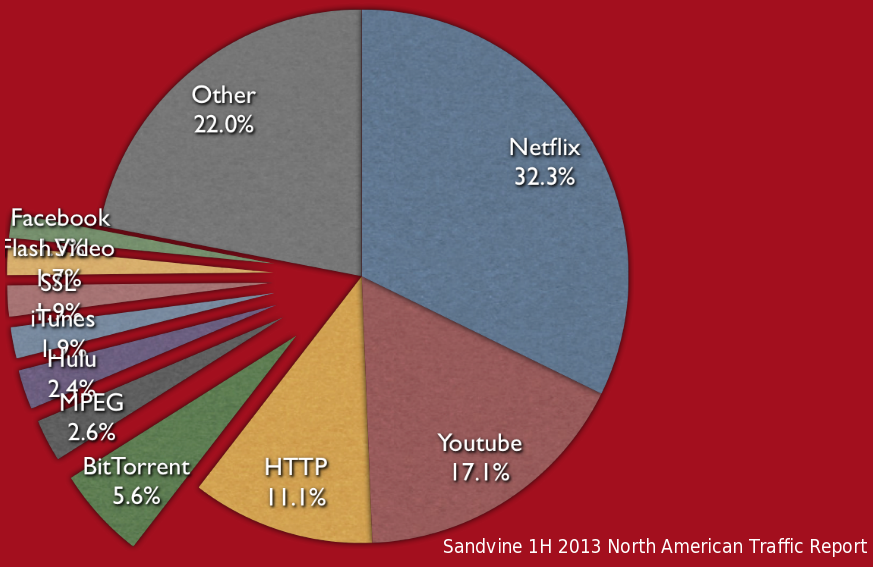
\includegraphics[width=11cm]{img/pie.png}
\end{center}
\end{frame}



\begin{frame}
\frametitle{FreeBSD developers}
\begin{figure}
\begin{tikzpicture}[
	foo/.style = { draw, circle }]

  \draw (0,0) circle[x radius=5.5cm, y radius=3.5cm];
  \draw (0,-2.5) node {contributors (thousands of 'em)};
  \draw (0,1) circle[x radius=4cm, y radius=2.5cm];
  \draw (0,-0.5) node {committers (\~{}400)};
  \draw (0,1) node[foo]{core (9)};
  \draw (-2,1) node[foo]{doceng};
  \draw (2,1) node[foo]{portmgr};
  \draw (-1,2) node[foo]{releng};
  \draw (1,2) node[foo]{secteam};
  \draw (-3.2,-1) node[foo]{vendors};
\end{tikzpicture}
\end{figure}
\end{frame}



\begin{frame}
\frametitle{Development workflow}
\begin{figure}
\begin{tikzpicture}[
	balloon/.style = { draw, minimum size=6mm, rounded corners=3mm,
			very thick,draw=black!50, top color=white,
			bottom color=black!20, font=\ttfamily,
			align=center },
	abovestr/.style = { midway, sloped, above }]

  \draw (0,0) node[name=dots, balloon]{\ldots};
  \draw (1,0) node[name=br9]{};
  \draw [fill] (node cs:name=br9) circle[radius=0.1cm];
  \draw (3,0) node[name=br10]{};
  \draw [fill] (node cs:name=br10) circle[radius=0.1cm];
  \node[name=current, balloon, right=7cm of dots]{FreeBSD CURRENT};
  \draw [->] (dots) -- (current) node [name=head, abovestr] {head};

  \node[name=st10, balloon, below left=1cm and 0.1 cm of current.center]
	{FreeBSD 10-STABLE};
  \draw [->] (br10) .. controls +(down:1cm) and +(left:1cm) ..
	 node[above,sloped] {stable/10} (st10.west);

  \node[name=br90, below left=3cm and 0.5cm of br10.center]{};
  \draw [fill] (node cs:name=br90) circle[radius=0.1cm];
  \draw [->] (br9) .. controls +(down:2cm) and +(left:2cm) ..
	 node[below,sloped] {stable/9} (br90);
  \node[name=br91, right=of br90]{};
  \draw [fill] (node cs:name=br91) circle[radius=0.1cm];
  \node[name=br92, right=of br91]{};
  \draw [fill] (node cs:name=br92) circle[radius=0.1cm];
  \node[name=st9, balloon, right=of br92] {FreeBSD 9-STABLE};
  \draw [->] (br90) -- (st9.west);
  \node[name=r90, balloon, below right=1cm and 0 cm of br90]{9.0-RELEASE};
  \draw [->] (br90.center) -- (r90);
  \node[name=r91, balloon, right=0.2cm of r90]{9.1-RELEASE};
  \draw [->] (br91) -- (r91);
  \node[name=r92, balloon, right=0.2cm of r91]{9.2-RELEASE};
  \draw [->] (br92) -- (r92);
\end{tikzpicture}
\end{figure}
\end{frame}



% OS #1
\begin{frame}
\frametitle{What an OS actually is?}
\begin{figure}
\begin{tikzpicture}[font=\Large, node distance = 0.1 cm, 
	block/.style = { rectangle, draw=black, thick, fill=white,
	inner xsep=0.5cm} ]

  \node [name=loader, block] { loader };
  \node [name=kernel, block,
	minimum height=1.5cm, minimum width=11cm, below=of loader] { kernel };
  \node [name=drivers, block, text centered,
	minimum height=1.3cm, right=2cm of kernel.center]
	{ drivers };
  \node [name=userland, block, minimum height=5cm, minimum width=11cm,
	below=of kernel] {};
  \node [below=of kernel] { userland };
\end{tikzpicture}
\end{figure}
\end{frame}

% OS #2
\begin{frame}
\frametitle{What an OS actually is?}
\begin{figure}
\begin{tikzpicture}[font=\Large, node distance = 0.1 cm, 
	block/.style = { rectangle, draw=black, thick, fill=white,
	inner xsep=0.5cm} ]

  \node [name=loader, block] { loader };
  \node [name=kernel, block,
	minimum height=1.5cm, minimum width=11cm, below=of loader] { kernel };
  \node [name=drivers, block, text centered,
	minimum height=1.3cm, right=2cm of kernel.center]
	{ drivers };
  \node [name=userland, block, minimum height=5cm, minimum width=11cm,
	below=of kernel] {};
  \node [below=of kernel] { userland };
  \node [name=sysutil, block, minimum height=1.5cm, minimum width=5cm,
	above left=0.1cm and 0.1cm of userland.center] { system utilities };
\end{tikzpicture}
\end{figure}
\end{frame}

% OS #3
\begin{frame}
\frametitle{What an OS actually is?}
\begin{figure}
\begin{tikzpicture}[font=\Large, node distance = 0.1 cm, 
	block/.style = { rectangle, draw=black, thick, fill=white,
	inner xsep=0.5cm} ]

  \node [name=loader, block] { loader };
  \node [name=kernel, block,
	minimum height=1.5cm, minimum width=11cm, below=of loader] { kernel };
  \node [name=drivers, block, text centered,
	minimum height=1.3cm, right=2cm of kernel.center]
	{ drivers };
  \node [name=userland, block, minimum height=5cm, minimum width=11cm,
	below=of kernel] {};
  \node [below=of kernel] { userland };
  \node [name=sysutil, block, minimum height=1.5cm, minimum width=5cm,
	above left=0.1cm and 0.1cm of userland.center] { system utilities };
  \node [name=env, block, minimum height=1.5cm, minimum width=5cm,
	above right=0.1cm and 0.1cm of userland.center] { POSIX environment };
\end{tikzpicture}
\end{figure}
\end{frame}

% OS #4
\begin{frame}
\frametitle{What an OS actually is?}
\begin{figure}
\begin{tikzpicture}[font=\Large, node distance = 0.1 cm, 
	block/.style = { rectangle, draw=black, thick, fill=white,
	inner xsep=0.5cm} ]

  \node [name=loader, block] { loader };
  \node [name=kernel, block,
	minimum height=1.5cm, minimum width=11cm, below=of loader] { kernel };
  \node [name=drivers, block, text centered,
	minimum height=1.3cm, right=2cm of kernel.center]
	{ drivers };
  \node [name=userland, block, minimum height=5cm, minimum width=11cm,
	below=of kernel] {};
  \node [below=of kernel] { userland };
  \node [name=sysutil, block, minimum height=1.5cm, minimum width=5cm,
	above left=0.1cm and 0.1cm of userland.center] { system utilities };
  \node [name=env, block, minimum height=1.5cm, minimum width=5cm,
	above right=0.1cm and 0.1cm of userland.center] { POSIX environment };
  \node [name=gui, block, minimum height=1.5cm, minimum width=5cm,
	below left=0.1cm and 0.1cm of userland.center] { GUI };
  \node [name=pkg, block, minimum height=1.5cm, minimum width=5cm,
	below right=0.1cm and 0.1cm of userland.center] { packaging system };
\end{tikzpicture}
\end{figure}
\end{frame}

% OS #5
\begin{frame}
\frametitle{What an OS actually is?}
\begin{figure}
\begin{tikzpicture}[font=\Large, node distance = 0.1 cm, 
	block/.style = { rectangle, draw=black, thick, fill=white,
	inner xsep=0.5cm} ]

  \node [name=loader, block] { loader };
  \node [name=kernel, block,
	minimum height=1.5cm, minimum width=11cm, below=of loader] { kernel };
  \node [name=drivers, block, text centered,
	minimum height=1.3cm, right=2cm of kernel.center]
	{ drivers };
  \node [name=userland, block, minimum height=5cm, minimum width=11cm,
	below=of kernel] {};
  \node [below=of kernel] { userland };
  \node [name=sysutil, block, minimum height=1.5cm, minimum width=5cm,
	above left=0.1cm and 0.1cm of userland.center] { system utilities };
  \node [name=env, block, minimum height=1.5cm, minimum width=5cm,
	above right=0.1cm and 0.1cm of userland.center] { POSIX environment };
  \node [name=pkg, block, minimum height=1.5cm, minimum width=2.5cm,
	text width=2cm, text centered,
	below left=0.1cm and 0.1cm of userland.center] { packaging system };
  \node [name=gui, block, minimum height=1.5cm,
	left=of pkg] { GUI };
  \node [name=installer, block, minimum height=1.5cm, minimum width=2.5cm,
	below right=0.1cm and 0.1cm of userland.center] { installer };
  \node [name=doc, block, minimum height=1.5cm, minimum width=2.5cm,
	below right=0.1cm and 2.6cm of userland.center] { docs };
\end{tikzpicture}
\end{figure}
\end{frame}



\begin{frame}
\frametitle{Recommended literature}
\center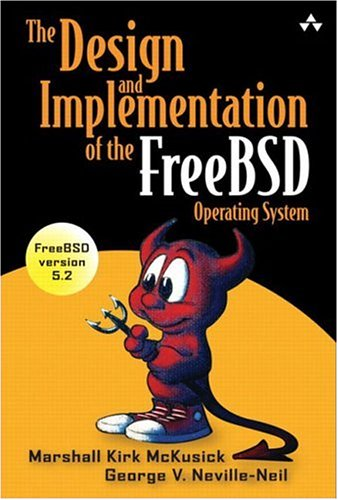
\includegraphics[height=3cm]{img/book_mcckusick.jpg}\\
The Design and Implementation of the FreeBSD Operating System,
\textit{Marshall Kirk McKusick, George V. Neville-Neil}, 2004 \\
\end{frame}

\begin{frame}
\frametitle{Recommended literature}
\begin{center}
\begin{tabular}{ p{3cm} p{6cm} }

\includegraphics[height=3cm]{img/book_unix.jpg} &
UNIX Network Programming,
\textit{W. Richard Stevens}, 2003 \\
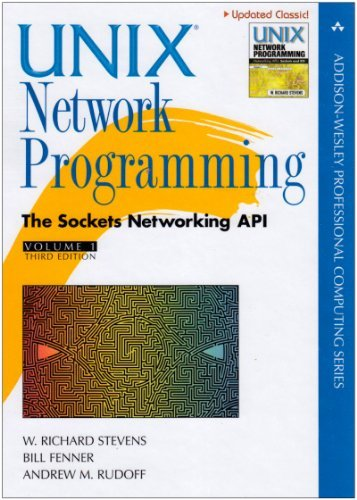
\includegraphics[height=3cm]{img/book_unp.jpg} &
Advanced Programming in the UNIX Environment,
\textit{W. Richard Stevens, Stephen A. Rago}, 2013
\end{tabular}
\end{center}
\end{frame}

\begin{frame}
\frametitle{Recommended literature}
\begin{center}
\begin{tabular}{ p{3cm} p{6cm} }
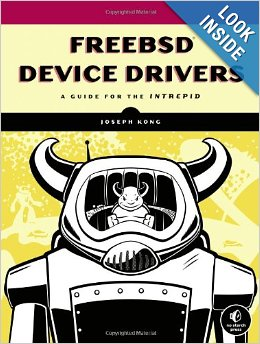
\includegraphics[height=3cm]{img/book_drivers.jpg} &
FreeBSD Device Drivers: A Guide for the Intrepid,
\textit{Kong, Joseph}, 2012 \\
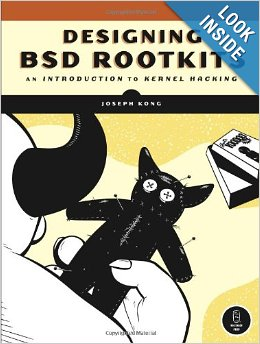
\includegraphics[height=3cm]{img/book_rootkits.jpg} &
Designing BSD Rootkits: An Introduction to Kernel Hacking,
\textit{Kong, Joseph}, 2009 \\
\end{tabular}
\end{center}
\end{frame}

\begin{frame}
\frametitle{Recommended literature}
\center
\includegraphics[height=3cm]{img/book_absolute.jpg}
Absolute FreeBSD: The Complete Guide to FreeBSD,
\textit{Lucas, Michael W.}, 2009 \\
\end{frame}

\end{document}
